\subsection{综合指标变化过程}\label{ch4:sec:process}

\begin{figure*}[ht!]
	\centering
	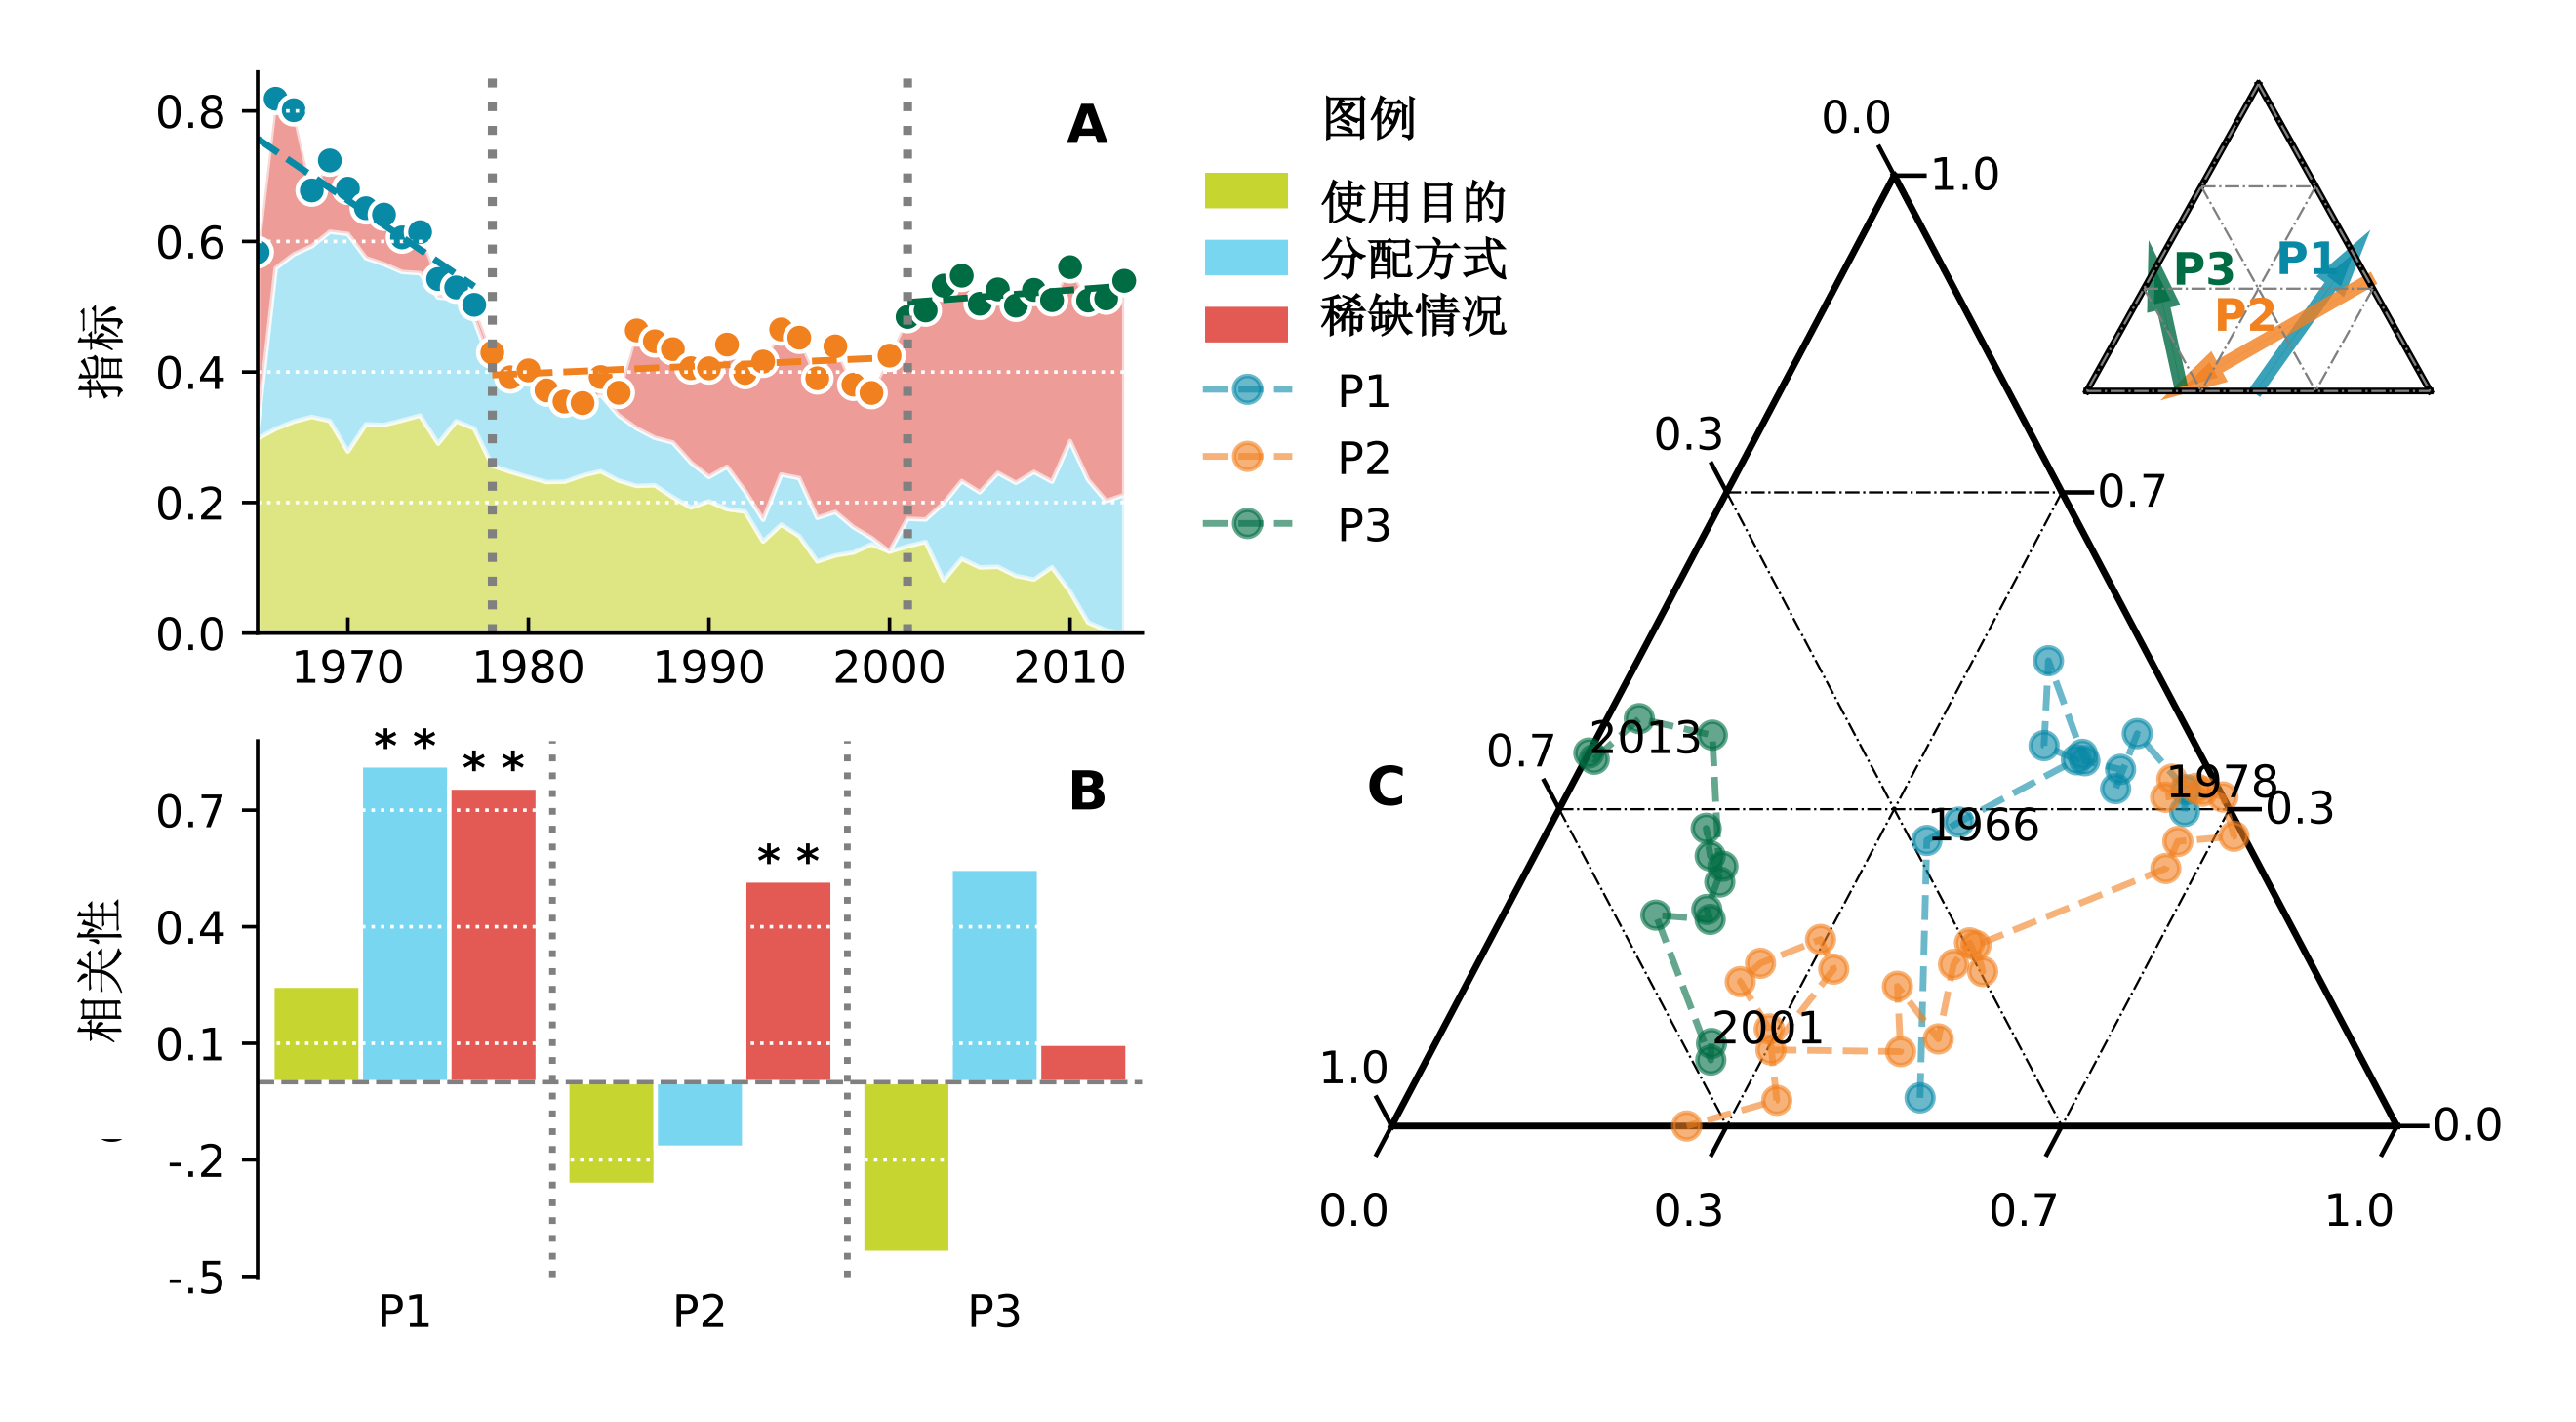
\includegraphics[width=\textwidth]{img/ch4/ch4_index.png}
	\caption[IWGI指数反映黄河流域的水治理变化阶段]{IWGI指数反映黄河流域的水治理变化阶段。两个突变点将1965年以来的黄河流域水治理划分为三个阶段,第一阶段(P1): $1965 \sim 1978$,第二阶段(P2): $1979 \sim 2001$,第三阶段(P3): $2002 \sim 2013$。
	\textbf{A,} 检测IWGI的突变点和三个指标的各自贡献:“稀缺情况(S)”、“使用目的(P)”和“分配方式(A)”。1978年和2001年出现了两个显著的变化点($p<0.01$)。
	\textbf{B,}  各阶段的IWGI变化与三个指标各自变化的相关性。
	\textbf{C,} IWGI随时间变化的同时,三个指标贡献比例的组合不断改变,致使水治理向不同方向发生阶段性转移。
	}\label{ch4:fig:IWGI}
\end{figure*}

IWGI在研究时段内存在两个突变点,将1965年以来的黄河流域水治理划分为三个阶段,第一阶段(P1): $1965 \sim 1978$,第二阶段(P2): $1979 \sim 2001$,第三阶段(P3): $2002 \sim 2013$,而“稀缺情况(S)”、“使用目的(P)”和“分配方式(A)”的三个指标在每个阶段的贡献不同(图~\ref{ch4:fig:IWGI}A)。
% 第一阶段
在第一个时期(P1, $1965 \sim 1978$)水资源压力对IWGI的贡献很小,“使用目的”和“分配方式”的指标的贡献更大(平均分别为$49.45\%$和$34.95\%$),但均呈现出显著的下降趋势($p<0.01$,图~\ref{ch4:fig:IWGI}~B),导致此时期IWGI迅速下降。
% 第二阶段
在第二阶段(P2, $1979 \sim 2001$),水资源压力指标的显著增加($p<0.01$)并为IWGI的略微上升做出主要贡献($p<0.01$,图~\ref{ch4:fig:IWGI}~A),而“使用目的”和“分配方式”的指标对IWGI的变化起了消极作用。
% 第三阶段
最后,在第三个时期(P3, $1995 \sim 2013$),尽管水资源压力指标在贡献中保持着$57.11\%$的最突出份额,但其数值已几乎保持不变,反而是“使用目的”的指标的降低和“分配方式”指标的增加,共同推动了综合指标IWGI的变化。
%的整体
综上所述,“稀缺情况(S)”、“使用目的(P)”和“分配方式(A)”的三个指标在不同时期对黄河流域水治理整体特征变化的贡献不同,将其演变历史划分为明显的三个阶段,依据其各自特点可命名为:集中供水时期、治理转变时期、适应增强时期(对应时间阶段分别为$1965 \sim 1978$、$1979 \sim 2001$、$2002 \sim 2013$(图~\ref{ch4:fig:IWGI}~C)。

\subsection{稀缺情况指标变化}

构成稀缺情况的指标(SFV指数)在研究时段(包括三个不同时期)内呈现出先降低、然后迅速增加、最后再次略微降低的变化趋势(图~\ref{ch4:fig:scarcity}~A)。
% ,表明水资源压力先减少再迅速增加,后趋于稳定
源区、上游、中游、下游这四个不同的区域中(图~\ref{ch4:fig:scarcity}~B),源区对三个时段的SFV指标变化几乎没有贡献,下游也仅在治理转变时期和适应增强时期呈现微弱的负向贡献。
对稀缺情况影响最大的是黄河的上游和中游,上游在集中供水时期和治理转变时期都是SFV变化的最大贡献区域,中游则在适应增强时期做出最大贡献。

\begin{figure}[!h]
  \centering
  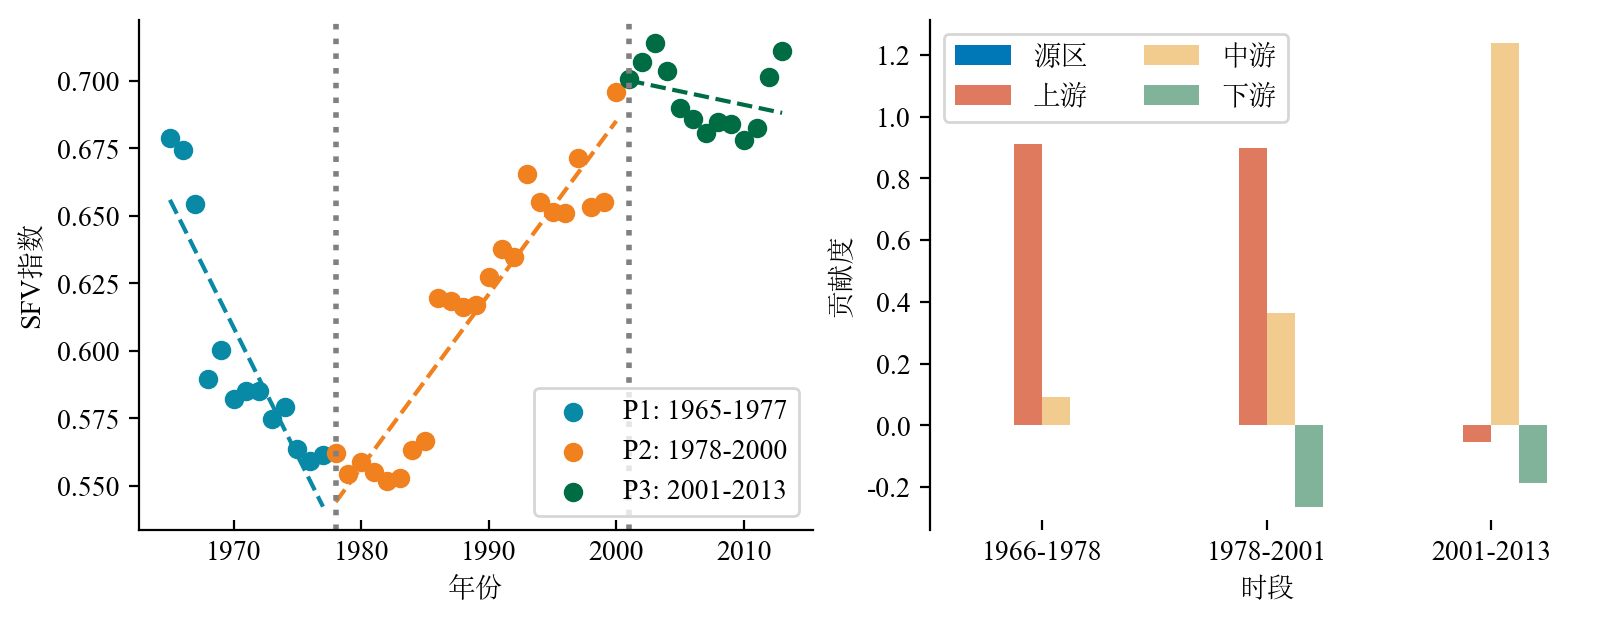
\includegraphics[width=\textwidth]{img/ch4/ch4_scarcity.png}
  \caption{稀缺性SFV指标变化趋势及各区域贡献}\label{ch4:fig:scarcity}
\end{figure}


\subsection{使用目的指标变化}

在用水目的上,供给性用水比例在集中供水时期基本保持不变,但在治理转变时期和适应增强时期呈现迅速下降的趋势(图\ref{ch4:fig:priority}~A)。
三个时段都是由灌溉用水的变化主导了该比例变化,城市、农村的人居用水、农村牲畜用水等几乎对该比例的变化没有影响(图\ref{ch4:fig:allocation}~B)。

\begin{figure}[!h]
	\centering
	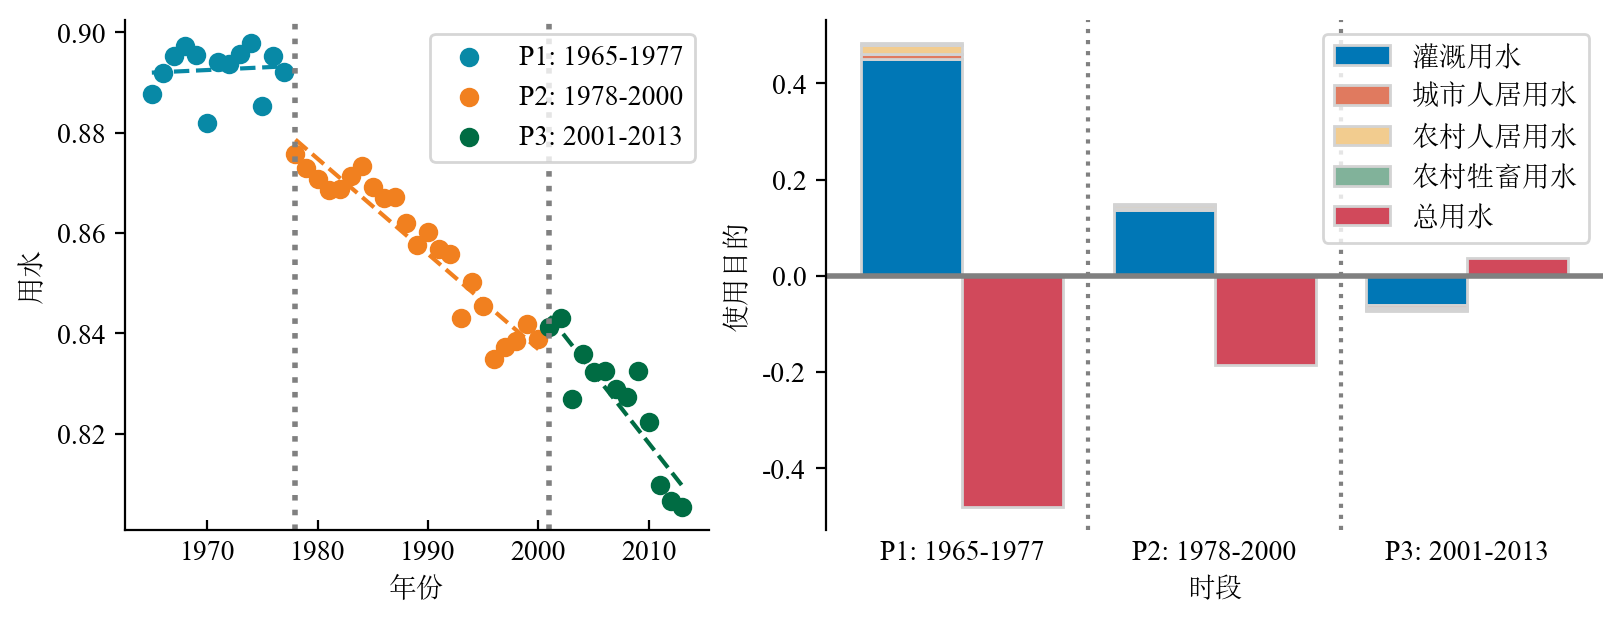
\includegraphics[width=\textwidth]{img/ch4/ch4_priority.png}
	\caption{供给性用水所占比例的变化趋势及各部门贡献}\label{ch4:fig:priority}
\end{figure}

\subsection{分配方式指标变化}

分配方式的指标变化呈现明显“V形”趋势,表明黄河的源区、上游、中游、下游之间水资源呈现先逐渐远离均匀分配,又在2000年后逐渐趋于平均的变化过程(图\ref{ch4:fig:allocation})。

\begin{figure}[!h]
	\centering
	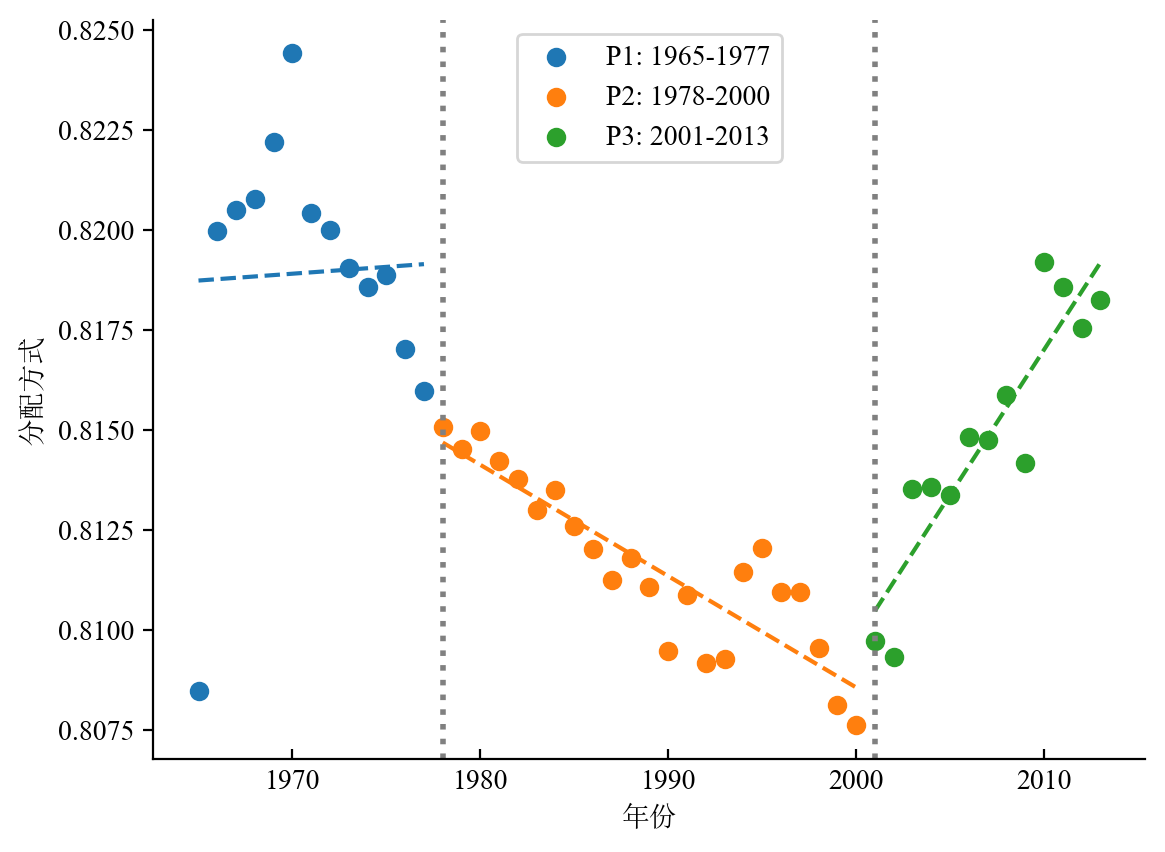
\includegraphics[width=0.6\textwidth]{img/ch4/ch4_allocation.png}
	\caption{分配方式指标的变化趋势}\label{ch4:fig:allocation}
\end{figure}